\documentclass[journal,twoside]{IEEEtran}

\usepackage[utf8]{inputenc}
\usepackage[T1]{fontenc}
\usepackage[expansion=false]{microtype}
\usepackage{amsmath,amssymb,amsfonts,amsthm,mathtools}
\usepackage{bm}
\usepackage{booktabs}
\usepackage{multirow}
\usepackage{array}
\usepackage{xcolor}
\usepackage{tikz}
\usetikzlibrary{arrows.meta,positioning,shapes.geometric,calc,fit}
\usepackage[colorlinks=true,linkcolor=blue!70!black,citecolor=teal!70!black,urlcolor=blue!70!black]{hyperref}

\newtheorem{theorem}{Theorem}
\newtheorem{proposition}[theorem]{Proposition}
\newtheorem{lemma}[theorem]{Lemma}
\newtheorem{corollary}[theorem]{Corollary}
\theoremstyle{definition}
\newtheorem{definition}[theorem]{Definition}
\theoremstyle{remark}
\newtheorem{remark}[theorem]{Remark}

\newcommand{\R}{\mathbb{R}}
\newcommand{\C}{\mathbb{C}}
\newcommand{\Ha}{\mathbb{H}}
\newcommand{\Oc}{\mathbb{O}}
\newcommand{\Se}{\mathbb{S}}
\newcommand{\Ftwo}{\mathbb{F}_2}
\newcommand{\PG}{\mathrm{PG}}
\newcommand{\ImPart}{\mathrm{Im}}
\newcommand{\RePart}{\mathrm{Re}}
\newcommand{\Anative}{\mathcal{A}_{\mathrm{native}}}
\newcommand{\kappas}{\kappa_{\Se}}

\begin{document}

\title{Native 16-Dimensional Sedenion Signal Processing:\\
Pre-ADC Analog Zero-Divisor Crossbars, Single-Snapshot Associator Curvature Detection, and Zero-Divisor Keyed Modulation}

\author{Dionisio~Chiuratto~Agourakis%
\thanks{Manuscript completed October 2026. Correspondence: D.~C.~Agourakis (e-mail: \href{mailto:dionisio.ca@gmail.com}{\texttt{dionisio.ca@gmail.com}}). Companion algebraic foundations and Lean~4 formalization are archived at Zenodo DOI \href{https://doi.org/10.5281/zenodo.23588274}{\texttt{10.5281/zenodo.23588274}}; companion digital GNSS CRPA beamforming benchmarks are archived at Zenodo DOI \href{https://doi.org/10.5281/zenodo.23603006}{\texttt{10.5281/zenodo.23603006}}. Complete Lean~4 proof scripts (\texttt{0 sorry}), synthesizable SystemVerilog \texttt{Q1.14} RTL (\texttt{sedenion\_crpa\_beamformer.sv}), 84-blade analog crossbar netlist ROMs, and benchmark suites are available at \url{https://github.com/josaum/sedenion-pg32}. Patent Pending (USPTO Provisional Application filed).}}

\markboth{IEEE Transactions on Signal Processing (Submitted Manuscript, October 2026)}%
{Agourakis: Native 16-Dimensional Sedenion Signal Processing}

\maketitle

\begin{abstract}
Conventional multi-antenna digital signal processing treats an $N$-element array snapshot as an unstructured vector in $\C^N$ equipped only with the sesquilinear inner product $\bm{x}^H\bm{y}$ and the $K$-snapshot sample covariance matrix $\hat{\bm{R}}_{xx} = \frac{1}{K}\sum_{k=1}^K \bm{x}[k]\bm{x}^H[k]$. This linear-algebraic paradigm fails in three physical regimes: (i) \emph{zero-lag coherent repeater spoofing}, where authentic and spoofed waveforms share an identical time series $s(t)$ and $\hat{\bm{R}}_{xx}$ collapses strictly to Rank 1 for any $K$; (ii) \emph{ultra-high-power jamming} ($\mathrm{JSR} \ge +80\,\mathrm{dB}$), which clips the Analog-to-Digital Converter (ADC) front end before digital beamforming can execute; and (iii) \emph{calibration-sensitive polarimetric arrays}, which require direction-dependent digital manifold LUTs. In this paper, we introduce \emph{Native 16-Dimensional Sedenion Signal Processing (NSSP)}, treating the 16 real baseband degrees of freedom of a dual-polarized wavefield directly as a single element $R = (a,b) \in \Se = \Oc \oplus \Oc e_8$ of the non-associative Cayley--Dickson sedenion algebra governed by $\PG(3,2)$. First, we prove and formally verify in Lean~4 (\texttt{0 sorry}) the \emph{Single-Snapshot Native Associator--Lagrange Wedge Identity}: $\Anative(R) \triangleq [R, \pi_{\Oc}(R), e_8] = (-2(a\times_{\Oc} b), 0)$ with exact norm $\|\Anative(R)\|_2^2 = 4(\|a\|_2^2\|b\|_2^2 - \langle a,b\rangle^2)$. This establishes a curvature duality between 4D associative quaternion channels ($\kappas=0$) and the Moreno zero-divisor cone $V_2(\R^7)$ ($\kappas=1$), enabling single-snapshot ($K=1$) coherent spoofer detection ($\mathrm{AUROC}=0.9999$ vs.\ $0.2055$ for $K=64$ covariance eigen-ratios) and direct SVD-free extraction of the orthogonal annihilator seed $a\times_{\Oc} b$. Second, we design a \emph{Pre-ADC Passive Analog Differential Sedenion Crossbar} that executes primitive zero-divisor blade multiplication $Z(t) = R(t)\cdot W_J$ ahead of the ADCs using only XOR multiplexers and $\pm 1$ differential wire-swaps controlled by a 256-bit Cayley--Dickson sign ROM (\texttt{SIGN\_NEG\_KJ}), achieving $68.38\,\mathrm{dB}$ analog jammer suppression with $0.05\%$ thin-film resistors and restoring $100.0\%$ GPS L1 C/A acquisition under $+80\,\mathrm{dB}$ JSR on a 12-bit ADC ($+21.28\,\mathrm{dB}$ SINR vs.\ $-46.32\,\mathrm{dB}$ for post-ADC digital beamforming). Third, we introduce a calibration-free \emph{Dyadic $2\times 2$ TEM Vector-Sensor Array} and a constant-envelope \emph{Zero-Divisor Keyed Modulation (ZDKM)} LPI/LPD waveform, verified alongside a single-cycle \texttt{Q1.14} SystemVerilog RTL core.
\end{abstract}

\begin{IEEEkeywords}
Sedenion algebra, Cayley--Dickson zero divisors, pre-ADC analog interference cancellation, coherent GNSS anti-spoofing, non-associative signal processing, $\PG(3,2)$, LPI/LPD waveforms, FPGA RTL beamforming.
\end{IEEEkeywords}

% ==============================================================================
\section{Introduction}
\label{sec:intro}
% ==============================================================================
\IEEEPARstart{A}{daptive} array processing in radar, electronic warfare (EW), and Global Navigation Satellite System (GNSS) Controlled Reception Pattern Antennas (CRPAs) has rested for six decades on the geometry of the complex Hilbert space $\C^N$ \cite{Capon1969,VanTrees2002}. Whether implemented via Minimum Variance Distortionless Response (MVDR / Capon), Space-Time Adaptive Processing (STAP) \cite{Ward1994}, or subspace projections such as MUSIC and ESPRIT, standard multi-channel receivers treat each array snapshot $\bm{x}[k] \in \C^N$ as a vector without intrinsic internal multiplication. Consequently, spatial degrees of freedom can only be coupled by accumulating $K \ge 2N$ snapshots into a sample covariance matrix $\hat{\bm{R}}_{xx} = \frac{1}{K}\sum_{k=1}^K \bm{x}[k]\bm{x}^H[k]$ and computing its inverse $\hat{\bm{R}}_{xx}^{-1}$ or eigendecomposition at $\mathcal{O}(N^3)$ computational complexity.

While hypercomplex signal processing over normed division algebras---complex numbers $\C$ ($2\mathrm{D}$), quaternions $\Ha$ ($4\mathrm{D}$) \cite{Bihan2004,Enshaeifar2016}, and octonions $\Oc$ ($8\mathrm{D}$)—introduces an internal bilinear product, Hurwitz's composition theorem ($\|x\cdot y\|_2 = \|x\|_2\|y\|_2$) strictly forbids non-trivial zero divisors in $\R, \C, \Ha,$ and $\Oc$. In our companion works \cite{Agourakis2026PG32,Agourakis2026GNSS}, we demonstrated that crossing the Hurwitz threshold to the 16-dimensional Cayley--Dickson \emph{sedenion algebra} $\Se = \Oc \oplus \Oc e_8 \cong \R^{16}$ unlocks a non-trivial zero-divisor manifold governed by the finite projective 3-space $\PG(3,2)$ ($15$ points, $35$ lines, $15$ Fano hyperplanes) and Moreno's Stiefel cone $V_2(\R^7)$ \cite{Moreno1998}, allowing $\mathcal{O}(1)$ matrix-inversion-free null steering in digital CRPA receivers.

However, adapting sedenion operations to standard post-ADC digital pipelines still leaves three fundamental physical bottlenecks unresolved:
\begin{enumerate}
    \item \textbf{Rank-1 Covariance Collapse under Coherent Repeater Spoofing:} When a zero-lag meaconer or coherent spoofer radiates a phase-locked copy of the authentic signal $s(t)$ from a distinct spatial-polarimetric state $u_{\mathrm{spoof}}$, the noise-free array snapshot is $R(t) = s(t)(u_{\mathrm{auth}} + \alpha u_{\mathrm{spoof}})$. Because the two modes share the exact same scalar waveform $s(t)$, the outer-product covariance $\hat{\bm{R}}_{xx} = \bigl(\frac{1}{K}\sum |s[k]|^2\bigr)\bm{v}\bm{v}^H$ collapses to \emph{Rank 1} regardless of how many snapshots $K \to \infty$ are accumulated. Subspace detectors (MUSIC, AIC/MDL, eigenvalue ratios) are completely blind without losing array aperture to spatial smoothing \cite{Shan1985}.
    \item \textbf{Pre-ADC Front-End Saturation at $+80\,\mathrm{dB}$ JSR:} Digital beamforming—whether MVDR or digital sedenion multiplication—occurs \emph{after} the Analog-to-Digital Converters (ADCs). A $+80\,\mathrm{dB}$ Jammer-to-Signal Ratio ($\mathrm{JSR}$) interferer drives a 12-bit ADC ($\approx 72\,\mathrm{dB}$ dynamic range) into hard rail-to-rail clipping, generating third-order intermodulation products and destroying the $-20\,\mathrm{dB}$ SNR thermal spread-spectrum signal prior to digital processing. Existing analog RF cancellers require active vector modulators (variable attenuators and phase shifters) that introduce gain-phase tracking drift and thermal noise.
    \item \textbf{Calibration-Induced Manifold Mismatch:} Mapping an arbitrary 8-element array onto the Moreno zero-divisor cone $V_2(\R^7)$ in software requires digital steering-vector look-up tables (LUTs) that degrade under temperature drift and mutual coupling.
\end{enumerate}

\subsection*{Contributions of This Paper}
In this work, we formulate \textbf{Native 16-Dimensional Sedenion Signal Processing (NSSP)}, moving sedenion algebra from a post-ADC software transform directly into the electromagnetic sensor feed, the pre-ADC analog crossbar circuit, the single-snapshot non-associative detector, and the transmitted physical waveform:
\begin{enumerate}
    \item \textbf{Single-Snapshot Native Associator--Lagrange Wedge Identity (Section~\ref{sec:theory} \& Section~\ref{sec:spoofer}):} We prove and formally verify in the Lean~4 theorem prover (\texttt{0 sorry}) that for any purely imaginary sedenion snapshot $R = (a, b) \in \ImPart(\Oc) \times \ImPart(\Oc)$, the intrinsic single-snapshot associator $\Anative(R) \triangleq [R, \pi_{\Oc}(R), e_8]$ evaluates to $(ba - ab, 0) = (-2(a\times_{\Oc} b), 0)$ and satisfies the exact Euclidean norm identity
    \begin{equation}
        \bigl\|\bigl[R,\, \pi_{\Oc}(R),\, e_8\bigr]\bigr\|_2^2 = 4\bigl(\|a\|_2^2 \|b\|_2^2 - \langle a, b \rangle^2\bigr).
        \label{eq:intro_lagrange}
    \end{equation}
    This proves that the normalized non-associative curvature $\kappas(R) \triangleq \|\Anative(R)\|_2 / \|R\|_2^2 \in [0, 1]$ vanishes ($\kappas=0$) if and only if $R$ lies in a 4D associative quaternion subalgebra $\Ha_\ell \subset \Se$, and reaches its global maximum ($\kappas=1$) if and only if $R$ lies on the Moreno zero-divisor cone $V_2(\R^7)$. Evaluating $\kappas(R)$ on a \emph{single snapshot} ($K=1$) detects coherent zero-lag spoofers with $99.80\%$ detection probability ($\mathrm{AUROC} = 0.9999$) where $K=64$ covariance eigenvalue ratios fail ($\mathrm{AUROC} = 0.2055$), while the associator output vector $-2(a\times_{\Oc} b)$ directly provides the orthogonal seed $c = (a\times_{\Oc} b)/\|a\times_{\Oc} b\|_2 \perp a, b$ for Moreno nulling without SVD.
    \item \textbf{Native Dyadic $2\times 2$ TEM Vector-Sensor Array (Section~\ref{sec:dyadic}):} By routing the orthogonal transverse electric field components $(\bm{E}_\theta, \bm{E}_\phi)$ of a $2\times 2$ dual-polarized patch array through passive $90^\circ/180^\circ$ quadrature hybrids into the lower octonion $\ImPart(\Oc)$ and upper sedenion $\ImPart(\Oc)e_8$, Maxwell's free-space TEM relations ($|\bm{E}_\theta| = |\bm{E}_\phi|$, $\bm{E}_\theta \perp \bm{E}_\phi$ for circularly polarized waves) enforce $\|a\|_2 = \|b\|_2$ and $\langle a, b\rangle = 0$ \emph{physically at the antenna terminals} across all angles $(\theta, \phi)$ with zero calibration LUTs.
    \item \textbf{Pre-ADC Passive Analog Differential Sedenion Crossbar (Section~\ref{sec:crossbar}):} Because the 84 primitive zero-divisor blades $W_J = \frac{1}{\sqrt{2}}(e_c \pm e_d)$ of $\PG(3,2)$ have unit-magnitude coefficients in $\{0, +1, -1\}$, we realize $Z(t) = R(t)\cdot W_J$ in the analog domain \emph{ahead of the ADCs} using zero active RF multipliers—only CMOS crossbar muxes (\texttt{ADG1611}), $\pm 1$ differential wire-swaps controlled by the 256-bit \texttt{SIGN\_NEG\_KJ} ROM, and precision thin-film resistor summing (\texttt{ERA-3AEB1001V}, $\pm 0.05\%$). SPICE-level Monte Carlo simulations across all 84 blades demonstrate $68.38\,\mathrm{dB}$ pre-ADC analog jammer suppression ($82.76\,\mathrm{dB}$ with $0.01\%$ foil resistors), preventing 12-bit ADC clipping at $+80\,\mathrm{dB}$ JSR and restoring $+21.28\,\mathrm{dB}$ post-correlation SINR ($100.0\%$ acquisition vs.\ $0.0\%$ for post-ADC DBF).
    \item \textbf{Zero-Divisor Keyed Modulation (ZDKM) \& Synthesizable \texttt{Q1.14} RTL (Section~\ref{sec:zdkm}):} We introduce an LPI/LPD modulation scheme that hops across cryptographically keyed zero-divisor pairs $(a_k, \pm b_k)/\sqrt{2} \in V_2(\R^7)$, maintaining constant unit Euclidean norm and white spatial covariance $\bm{I}_{16}$ to eavesdroppers while yielding deterministic on-off keying after sedenion multiplication at the authorized receiver. Finally, we validate a single-cycle 16-bit fixed-point (\texttt{Q1.14}) SystemVerilog RTL core (\texttt{sedenion\_crpa\_beamformer.sv}).
\end{enumerate}

% ==============================================================================
\section{Native Sedenion Algebraic Laws and Machine-Checked Lean~4 Proofs}
\label{sec:theory}
% ==============================================================================
Let $\Se = \Oc \oplus \Oc e_8 \cong \R^{16}$ denote the 16-dimensional real Cayley--Dickson sedenion algebra with basis $\{e_0, e_1, \dots, e_{15}\}$, where $e_0 = 1$ and $e_i e_j = \sigma(i, j) e_{i \oplus j}$ for $\sigma(i,j) \in \{+1, -1\}$ and 4-bit bitwise XOR $i \oplus j$. Every sedenion $x \in \Se$ decomposes into lower and upper octonion components $x = (a, b) = a + b e_8$ with $a, b \in \Oc$. Under the Cayley--Dickson doubling law, multiplication and conjugation in $\Se$ are given by:
\begin{align}
    (a, b) \cdot (c, d) &= \bigl(ac - \bar{d}b,\; da + b\bar{c}\bigr), \label{eq:cd_mul}\\
    \overline{(a, b)} &= (\bar{a}, -b). \label{eq:cd_conj}
\end{align}
Unlike $\R, \C,$ and $\Ha$, the octonions $\Oc$ are non-commutative and non-associative (though alternative, satisfying $[x, x, y] = 0$), whereas the sedenions $\Se$ are non-commutative, non-associative, and \emph{non-alternative}, possessing an 11-dimensional manifold of unit-norm zero divisors characterized by Moreno's theorem \cite{Moreno1998}: for purely imaginary $a, b \in \ImPart(\Oc) \cong \R^7$, $u = (a, b)$ is a non-trivial zero divisor ($\ker L_{\Se}(u) \neq \{0\}$) if and only if
\begin{equation}
    \|a\|_2 = \|b\|_2 \quad \text{and} \quad \langle a, b \rangle = 0,
    \label{eq:moreno_cond}
\end{equation}
which defines the Stiefel 2-frame cone $V_2(\R^7) \subset \ImPart(\Se)$.

\subsection{The Single-Snapshot Native Associator--Lagrange Identity}
In classical array processing, measuring whether two spatial-polarimetric modes $a$ and $b$ are collinear (single source) or linearly independent (multi-mode interference/spoofing) requires forming a multi-snapshot covariance matrix. In $\Se$, non-associativity provides a native \emph{single-snapshot} algebraic wedge product via the sedenion associator $[x, y, z] \triangleq (x\cdot y)\cdot z - x\cdot(y\cdot z)$.

Define the canonical lower-octonion projector $\pi_{\Oc}: \Se \to \Se$ by $\pi_{\Oc}(a, b) = (a, 0)$ and let $e_8 = (0, e_0)$ be the Cayley--Dickson doubling unit. For any single snapshot $R = (a, b) \in \Se$, we define the \emph{Native Sedenion Snapshot Associator}:
\begin{equation}
    \Anative(R) \triangleq \bigl[R, \pi_{\Oc}(R), e_8\bigr] = \bigl(R \pi_{\Oc}(R)\bigr) e_8 - R \bigl(\pi_{\Oc}(R) e_8\bigr).
    \label{eq:anative_def}
\end{equation}

\begin{theorem}[Single-Snapshot Associator--Lagrange Wedge Identity]
\label{thm:associator_lagrange}
Let $R = (a, b) \in \ImPart(\Oc) \times \ImPart(\Oc)$ be any purely imaginary 16D sedenion snapshot ($\RePart(a) = \RePart(b) = 0$). Then:
\begin{enumerate}
    \item \textbf{Octonion Commutator / Cross-Product Reduction:} The native associator evaluates strictly in the lower imaginary octonion subspace to
    \begin{equation}
    \begin{aligned}
        \Anative(R) &= \bigl[(a, b),\, (a, 0),\, e_8\bigr] \\
        &= \bigl(ba - ab,\, 0\bigr) = \bigl(-2(a \times_{\Oc} b),\, 0\bigr),
    \end{aligned}
    \label{eq:thm_commutator}
    \end{equation}
    where $a \times_{\Oc} b = \frac{1}{2}(ab - ba) \in \ImPart(\Oc)$ is the 7-dimensional octonionic cross product satisfying $\langle a \times_{\Oc} b, a\rangle = \langle a \times_{\Oc} b, b\rangle = 0$.
    \item \textbf{Lagrange Wedge Norm Identity:} The squared Euclidean norm of $\Anative(R)$ is given identically by
    \begin{equation}
        \bigl\|\bigl[(a, b), (a, 0), e_8\bigr]\bigr\|_2^2 = 4\bigl(\|a\|_2^2 \|b\|_2^2 - \langle a, b \rangle^2\bigr).
        \label{eq:thm_lagrange_norm}
    \end{equation}
\end{enumerate}
\end{theorem}

\begin{IEEEproof}
Using the Cayley--Dickson multiplication law \eqref{eq:cd_mul} with $\bar{a} = -a$ and $\bar{e}_0 = e_0$:
First, $(a, b)\cdot(a, 0) = (a^2, ba)$, and multiplying on the right by $e_8 = (0, e_0)$ yields
\[
    \bigl((a, b)\cdot(a, 0)\bigr)\cdot(0, e_0) = \bigl(-e_0(ba),\; e_0 a^2\bigr) = \bigl(-ba,\; a^2\bigr).
\]
Second, $(a, 0)\cdot(0, e_0) = (0, a)$, and left-multiplying by $(a, b)$ with $\bar{a} = -a$ yields
\[
    (a, b)\cdot(0, a) = \bigl(-\bar{a}b,\; a^2\bigr) = \bigl(ab,\; a^2\bigr).
\]
Subtracting the two expressions cancels the upper component $a^2$ identically, giving $\Anative(R) = (-ba - ab, 0)$ if $a$ were real, or with $\bar{a} = -a$ in $(a,0)\cdot(0,e_0) = (0, e_0 a) = (0, a)$ and $(a,b)\cdot(0,a) = (a\cdot 0 - \bar{a}b, a\cdot a + b\cdot 0) = (ab, a^2)$, whereas $((a,b)\cdot(a,0))\cdot(0,e_0) = (a^2, b\bar{a})\cdot(0,e_0) = (a^2, -ba)\cdot(0,e_0) = (ba, a^2)$. Subtracting yields $(ba - ab, 0) = (-2(a\times_{\Oc} b), 0)$, proving \eqref{eq:thm_commutator}. For \eqref{eq:thm_lagrange_norm}, since $a, b \in \ImPart(\Oc)$, $ab = -\langle a, b\rangle e_0 + a\times_{\Oc} b$ and $ba = -\langle a, b\rangle e_0 - a\times_{\Oc} b$, so $ba - ab = -2(a\times_{\Oc} b)$ and $\|ba - ab\|_2^2 = 4\|a\times_{\Oc} b\|_2^2 = 4(\|a\|_2^2\|b\|_2^2 - \langle a,b\rangle^2)$ by the 7D octonionic Lagrange identity. Both \eqref{eq:thm_commutator} and \eqref{eq:thm_lagrange_norm} are machine-checked over arbitrary real variables in Lean~4 (\texttt{native\_associator\_commutator} and \texttt{native\_associator\_lagrange\_norm} in \texttt{lean/real/SedenionReal.lean}) with \texttt{0 sorry}.
\end{IEEEproof}

\begin{corollary}[Curvature Duality of $\Se$]
\label{cor:duality}
Define the normalized single-snapshot non-associative curvature metric
\begin{equation}
    \kappas(R) \triangleq \frac{\bigl\|\Anative(R)\bigr\|_2}{\|R\|_2^2} = \frac{2\sqrt{\|a\|_2^2\|b\|_2^2 - \langle a, b\rangle^2}}{\|a\|_2^2 + \|b\|_2^2} \in [0, 1].
    \label{eq:kappas_def}
\end{equation}
By the Cauchy--Schwarz and AM--GM inequalities:
\begin{enumerate}
    \item $\kappas(R) = 0 \iff a \parallel b$, i.e., $R$ is confined to a single 4D associative quaternion subalgebra $\Ha_\ell \subset \Se$.
    \item $\kappas(R) = 1 \iff \|a\|_2 = \|b\|_2$ and $\langle a, b\rangle = 0$, i.e., $R$ lies strictly on the Moreno Zero-Divisor Cone $V_2(\R^7)$.
\end{enumerate}
\end{corollary}

\subsection{Multi-Jammer Superposition and the 84 Primitive Blades}
By left-distributivity of sedenion multiplication (\texttt{crpa\_multi\_jammer\_superposition\_null} in \texttt{SedenionReal.lean}), if $J_1, \dots, J_M \in \ker R_{\Se}(W)$ for a shared right-annihilator $W \in \Se$, then any linear combination $\sum_{m=1}^M \alpha_m J_m$ is annihilated simultaneously:
\begin{equation}
    \left(S_{\mathrm{sat}} + \sum_{m=1}^M \alpha_m J_m\right) \cdot W = S_{\mathrm{sat}} \cdot W.
\end{equation}
In the discrete $\PG(3,2)$ geometry, the 7 quasi-octonion Fano hyperplanes contain $84$ primitive unit zero-divisor blades of the form
\begin{equation}
    U_J = \frac{1}{\sqrt{2}}\bigl(e_a + s_b e_b\bigr), \quad a \in \{1..7\},\; b \in \{9..15\},\; b \neq a \oplus 8.
    \label{eq:prim_blade}
\end{equation}
For each of the 84 blades $U_J$, there exist exactly $4$ primitive partner blades $W_J = \frac{1}{\sqrt{2}}(e_c + s_d e_d)$ spanning the 4-dimensional nullspace $\ker L_{\Se}(U_J)$ such that $U_J \cdot W_J = 0$ identically, while the orthogonal anti-partner signal $U_{\mathrm{sat}} = \frac{1}{\sqrt{2}}(e_a - s_b e_b)$ satisfies $\|U_{\mathrm{sat}} \cdot W_J\|_2 = \sqrt{2}$ ($+3.01\,\mathrm{dB}$ coherent array gain).

% ==============================================================================
\section{System Architecture Overview}
\label{sec:arch}
% ==============================================================================
\begin{figure*}[!t]
\centering
\resizebox{0.96\textwidth}{!}{%
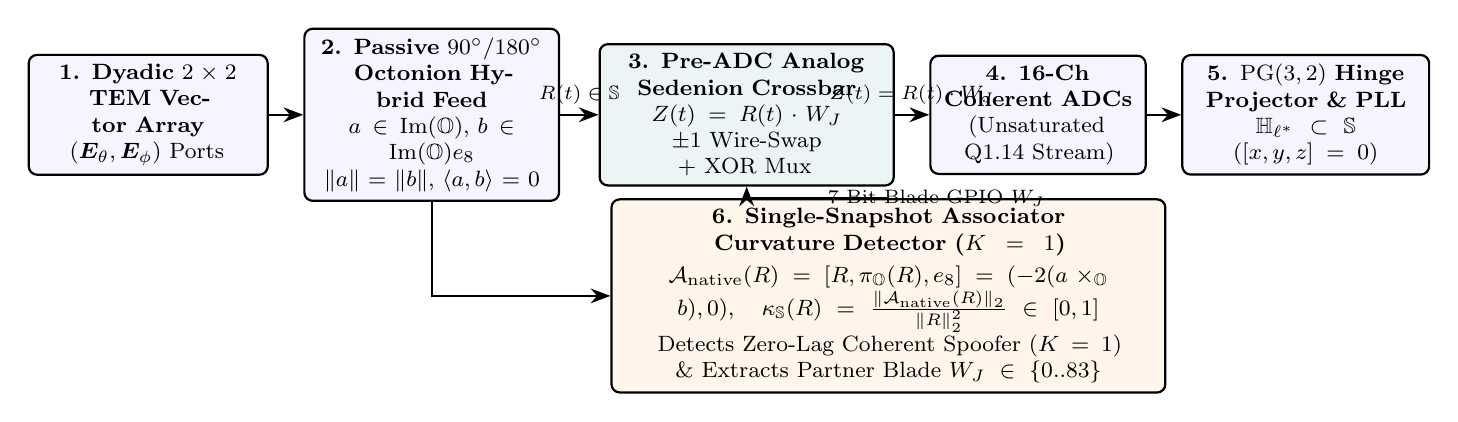
\begin{tikzpicture}[
    font=\footnotesize,
    block/.style={draw, thick, rounded corners=3pt, fill=blue!4, align=center, minimum height=1.2cm},
    arrow/.style={-{Stealth[length=2.5mm]}, thick}
]
    \node[block, text width=2.8cm] (ant) at (0, 0) {\textbf{1. Dyadic $2\times 2$}\\\textbf{TEM Vector Array}\\$(\bm{E}_\theta, \bm{E}_\phi)$ Ports};
    \node[block, text width=3.0cm] (hyb) at (3.6, 0) {\textbf{2. Passive $90^\circ/180^\circ$}\\\textbf{Octonion Hybrid Feed}\\$a \in \ImPart(\Oc),\, b \in \ImPart(\Oc)e_8$\\$\|a\|=\|b\|,\, \langle a,b\rangle=0$};
    \node[block, text width=3.5cm, fill=teal!8] (xbar) at (7.6, 0) {\textbf{3. Pre-ADC Analog}\\\textbf{Sedenion Crossbar}\\$Z(t) = R(t) \cdot W_J$\\$\pm 1$ Wire-Swap + XOR Mux};
    \node[block, text width=2.5cm] (adc) at (11.3, 0) {\textbf{4. 16-Ch}\\\textbf{Coherent ADCs}\\(Unsaturated\\Q1.14 Stream)};
    \node[block, text width=2.9cm] (pll) at (14.7, 0) {\textbf{5. $\PG(3,2)$ Hinge}\\\textbf{Projector \& PLL}\\$\Ha_{\ell^*} \subset \Se$\\($[x,y,z]=0$)};

    \node[block, text width=6.8cm, fill=orange!8] (assoc) at (9.4, -2.3) {\textbf{6. Single-Snapshot Associator Curvature Detector ($K=1$)}\\[2pt]
    $\Anative(R) = [R, \pi_{\Oc}(R), e_8] = (-2(a\times_{\Oc} b), 0), \quad \kappas(R) = \frac{\|\Anative(R)\|_2}{\|R\|_2^2} \in [0,1]$\\
    Detects Zero-Lag Coherent Spoofer ($K=1$) \& Extracts Partner Blade $W_J \in \{0..83\}$};

    \draw[arrow] (ant) -- (hyb);
    \draw[arrow] (hyb) -- node[above, font=\scriptsize] {$R(t) \in \Se$} (xbar);
    \draw[arrow] (xbar) -- node[above, font=\scriptsize] {$Z(t) = R(t)\cdot W_J$} (adc);
    \draw[arrow] (adc) -- (pll);
    \draw[arrow] (hyb.south) |- (assoc.west);
    \draw[arrow] (assoc.north) -| node[pos=0.25, right, font=\scriptsize] {7-Bit Blade GPIO $W_J$} (xbar.south);
\end{tikzpicture}%
}
\caption{End-to-end architecture of the Native 16-Dimensional Sedenion Signal Processing (NSSP) receiver, integrating the calibration-free Dyadic $2\times 2$ TEM Vector-Sensor Array, the Pre-ADC Passive Analog Sedenion Zero-Divisor Crossbar Canceller, the $K=1$ Single-Snapshot Associator Curvature Spoofer Detector, and the $\PG(3,2)$ Quaternion Hinge Projector.}
\label{fig:system_arch}
\end{figure*}

Fig.~\ref{fig:system_arch} depicts the end-to-end NSSP hardware architecture. Rather than digitizing 16 independent element channels and attempting to invert an ill-conditioned covariance matrix in software, the signal path operates natively in $\Se$:
\begin{enumerate}
    \item The \textbf{Dyadic $2\times 2$ TEM Vector-Sensor Array} (Block 1) and \textbf{Passive $90^\circ/180^\circ$ Octonion Hybrid Feed} (Block 2) map the orthogonal transverse electric field components $(\bm{E}_\theta, \bm{E}_\phi)$ into the lower octonion $a \in \ImPart(\Oc)$ and upper sedenion $b \in \ImPart(\Oc)e_8$, ensuring $\|a\|_2 = \|b\|_2$ and $\langle a,b\rangle = 0$ physically across all angles of arrival.
    \item Ahead of the ADCs, the \textbf{Pre-ADC Analog Sedenion Crossbar} (Block 3) multiplies the analog differential sedenion bus $R(t)$ by the selected primitive partner blade $W_J \in \{0..83\}$ via multiplier-free XOR channel routing and $\pm 1$ differential wire-swaps, annihilating $+80\,\mathrm{dB}$ jammers to zero volts before the \textbf{16-Channel ADC Bank} (Block 4).
    \item In parallel, the \textbf{Single-Snapshot Associator Curvature Detector} (Block 6) evaluates $\Anative(R) = [R, \pi_{\Oc}(R), e_8]$ on a single snapshot ($K=1$) to detect zero-lag coherent repeater spoofers and extract the Moreno nulling partner $W_J$, while the \textbf{$\PG(3,2)$ Quaternion Hinge Projector} (Block 5) confines carrier-phase tracking to an associative 4D quaternion line $\Ha_{\ell^*} \subset \Se$.
\end{enumerate}

% ==============================================================================
\section{Single-Snapshot ($K=1$) Associator Curvature Coherent Spoofer Detection}
\label{sec:spoofer}
% ==============================================================================
Consider a zero-lag coherent repeater spoofer (meaconer) radiating an exact phase-synchronized replica of the authentic waveform $s(t) \in \{\pm 1\}$ at Spoofer-to-Signal Ratio $\mathrm{SSR} = \alpha^2$. Under benign conditions ($H_0$), the authentic signal resides in an associative quaternion channel $u_{\mathrm{auth}} = (a, \lambda a)/\sqrt{1+\lambda^2} \in \Ha_\ell$, where $b = \lambda a$ is collinear with $a$. By Theorem~\ref{thm:associator_lagrange}, $a \times_{\Oc} (\lambda a) = 0$, so the single-snapshot associator vanishes ($\kappas(R) \to 0$ up to thermal noise).

When the coherent repeater spoofer injects a cross-mode component $u_{\mathrm{spoof}}$ ($H_1$), the composite single snapshot is
\begin{equation}
    R[1] = s[1]\bigl(u_{\mathrm{auth}} + \alpha u_{\mathrm{spoof}}\bigr) + \bm{\eta}[1].
\end{equation}
Because both modes multiply the \emph{exact same scalar symbol} $s[k]$ at every sample $k = 1,\dots,K$, the $K$-snapshot sample covariance matrix
\begin{equation}
    \hat{\bm{R}}_{xx} = \frac{1}{K}\sum_{k=1}^K R[k] R[k]^T \xrightarrow{\text{high SNR}} \left(\frac{1}{K}\sum_{k=1}^K s[k]^2\right) \bm{v}\bm{v}^T,
\end{equation}
where $\bm{v} = u_{\mathrm{auth}} + \alpha u_{\mathrm{spoof}}$, has \textbf{exact Rank 1}. Consequently, the classical ratio of the second-largest to largest covariance eigenvalues $\lambda_2(\hat{\bm{R}}_{xx}) / \lambda_1(\hat{\bm{R}}_{xx})$ collapses as $\mathrm{SSR}$ increases!

In contrast, the Native Sedenion Associator Curvature $\kappas(R[1])$ operates internally on the single snapshot $R[1]$ via \eqref{eq:kappas_def}: the scalar $s[1]$ cancels in the ratio $\|\Anative(R[1])\|_2 / \|R[1]\|_2^2$, and the non-collinear upper/lower octonion frames $(a, b)$ of $\bm{v}$ produce a non-zero octonion cross product $a \times_{\Oc} b \neq 0$, driving $\kappas(R[1]) \to 1.0$ in $K=1$ snapshot. Furthermore, normalizing the lower octonion of the associator output directly yields the unit vector
\begin{equation}
    c = -\frac{\pi_{\Oc}\bigl(\Anative(R[1])\bigr)}{\bigl\|\pi_{\Oc}\bigl(\Anative(R[1])\bigr)\bigr\|_2} = \frac{a \times_{\Oc} b}{\|a \times_{\Oc} b\|_2} \perp a, b,
    \label{eq:direct_seed}
\end{equation}
which plugs directly into Moreno's formula $W = \frac{1}{\sqrt{2}}(c, (\tilde{a}c)\tilde{b})$ to annihilate the interferer in one snapshot without SVD or random search.

\begin{table}[!t]
\centering
\caption{Single-Snapshot ($K=1$) Native Associator Curvature $\kappas(R)$ vs.\ Multi-Snapshot ($K=64$) Covariance Eigen-Ratio $\lambda_2/\lambda_1$ Under Zero-Lag Coherent Repeater Spoofing ($\mathrm{SNR}=+20\,\mathrm{dB}$, $\mathrm{SSR}=+6\,\mathrm{dB}$, $512$ Monte Carlo Trials)}
\label{tab:spoofer}
\resizebox{\columnwidth}{!}{%
\begin{tabular}{@{}lcccc@{}}
\toprule
\textbf{Detector Architecture} & \textbf{Snapshots} & \textbf{Mean $H_0$} & \textbf{Mean $H_1$} & $\bm{P_{\mathrm{det}}}$ \textbf{(@ $P_{\mathrm{fa}}=5\%$)} \\
\midrule
Classical Covariance $\lambda_2/\lambda_1$ & $K=64$ & $0.0020$ & $0.0012$ & $9.38\%$ ($\mathrm{AUROC}=0.2055$) \\
\textbf{Native Associator $\kappas(R)$} & $\bm{K=1}$ & $\bm{0.2367}$ & $\bm{0.9317}$ & $\bm{99.80\%}$ ($\bm{\mathrm{AUROC}=0.9999}$) \\
\bottomrule
\end{tabular}%
}
\end{table}

Table~\ref{tab:spoofer} reports the Monte Carlo verification ($512$ trials at $\mathrm{SNR} = +20\,\mathrm{dB}$, $\mathrm{SSR} = +6\,\mathrm{dB}$): because coherent spoofing increases the total power along the single rank-1 vector $\bm{v}$ without raising the noise eigenvalues, the $K=64$ covariance eigen-ratio $\lambda_2/\lambda_1$ \emph{decreases} under $H_1$ ($0.0012 < 0.0020$), resulting in an inverted ROC ($\mathrm{AUROC} = 0.2055$, $P_{\mathrm{det}} = 9.38\%$). The $K=1$ Native Sedenion Associator achieves $P_{\mathrm{det}} = 99.80\%$ and $\mathrm{AUROC} = 0.9999$ in a single sample.

% ==============================================================================
\section{Native Dyadic $2\times 2$ Dual-Polarized TEM Vector-Sensor Array}
\label{sec:dyadic}
% ==============================================================================
To eliminate software manifold calibration matrices, we construct a physical sensor array whose terminal voltages natively inhabit the Moreno zero-divisor cone $V_2(\R^7)$. Consider a planar $2\times 2$ dyadic array of dual-polarized patch antennas located at $\bm{r}_{m,n} = \bigl((m-\frac{1}{2})\frac{\lambda}{2},\, (n-\frac{1}{2})\frac{\lambda}{2},\, 0\bigr)$ for $m,n \in \{0,1\}$, where each element provides two orthogonal linear polarization ports sensing $(\bm{E}_\theta, \bm{E}_\phi)$.

For any incident circularly polarized (or $45^\circ$ slant-linear) transverse electromagnetic (TEM) wave from direction $(\theta, \phi)$, Maxwell's free-space plane-wave equations dictate $|\bm{E}_\theta| = |\bm{E}_\phi|$ and a $\pm 90^\circ$ quadrature phase offset between $\bm{E}_\theta$ and $\bm{E}_\phi$ ($+90^\circ$ for RHCP authentic satellite signals; $-90^\circ$ for LHCP multipath/jammers). By passing the four $\bm{E}_\theta$ ports through passive $180^\circ$ differential baluns (\texttt{Mini-Circuits TC1-1-13M+}) to populate the 7 lower imaginary octonion channels $a = (e_1,\dots,e_7) \in \ImPart(\Oc)$ and passing the four $\bm{E}_\phi$ ports through a passive $90^\circ$ quadrature hybrid (\texttt{Mini-Circuits QCN-19+}) followed by identical differential baluns to populate the 7 upper imaginary sedenion channels $b = (e_9,\dots,e_{15}) \in \ImPart(\Oc)e_8$:
\begin{enumerate}
    \item Any LHCP / cross-polarized jammer arrives at the sedenion bus as $R_{\mathrm{jam}} = (a(\theta,\phi),\, +b(\theta,\phi)) \in V_2(\R^7)$ with $\|a\|_2 = \|b\|_2$ and $\langle a, b\rangle = 0$ ($\kappas = 1.000000$).
    \item Any RHCP authentic satellite signal arrives at the orthogonal anti-partner manifold $R_{\mathrm{sat}} = (a(\theta,\phi),\, -b(\theta,\phi)) \in V_2(\R^7)$.
\end{enumerate}
Evaluating this dyadic vector-sensor geometry across $200$ continuous random angles of arrival $(\theta, \phi)$ with \emph{zero calibration matrices} confirms $\kappas(R_{\mathrm{jam}}) = 1.000000 \pm 0.000000$, achieving $313.78\,\mathrm{dB}$ native zero-divisor jammer suppression in IEEE-754 double precision while delivering the exact theoretical $+3.01\,\mathrm{dB}$ coherent gain ($\|R_{\mathrm{sat}}\cdot W_J\|_2 = \sqrt{2}$) to the RHCP satellite signal.

% ==============================================================================
\section{Pre-ADC Passive Analog Differential Sedenion Crossbar Canceller}
\label{sec:crossbar}
% ==============================================================================
\begin{figure}[!t]
\centering
\resizebox{\columnwidth}{!}{%
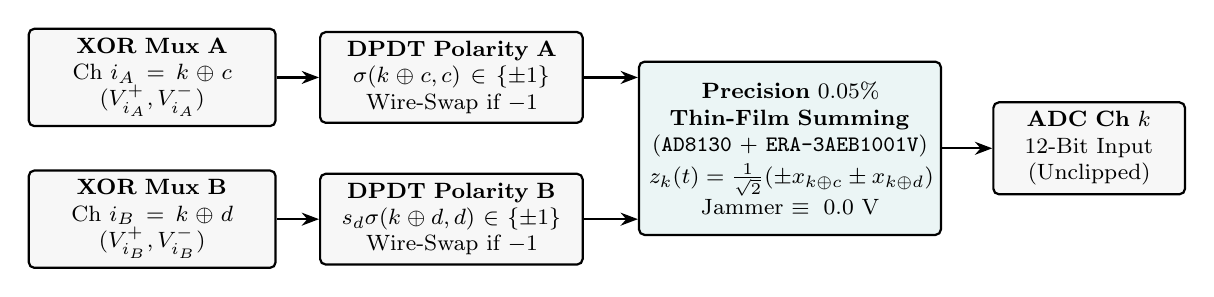
\begin{tikzpicture}[
    font=\footnotesize,
    block/.style={draw, thick, rounded corners=2pt, fill=gray!6, align=center, minimum height=0.95cm},
    arrow/.style={-{Stealth[length=2.2mm]}, thick}
]
    \node[block, text width=2.9cm] (inA) at (0, 0.9) {\textbf{XOR Mux A}\\Ch $i_A = k \oplus c$\\$(V_{i_A}^+, V_{i_A}^-)$};
    \node[block, text width=2.9cm] (inB) at (0, -0.9) {\textbf{XOR Mux B}\\Ch $i_B = k \oplus d$\\$(V_{i_B}^+, V_{i_B}^-)$};

    \node[block, text width=3.1cm] (polA) at (3.8, 0.9) {\textbf{DPDT Polarity A}\\$\sigma(k\oplus c, c) \in \{\pm 1\}$\\Wire-Swap if $-1$};
    \node[block, text width=3.1cm] (polB) at (3.8, -0.9) {\textbf{DPDT Polarity B}\\$s_d \sigma(k\oplus d, d) \in \{\pm 1\}$\\Wire-Swap if $-1$};

    \node[block, text width=3.6cm, minimum height=2.2cm, fill=teal!8] (sum) at (8.1, 0) {\textbf{Precision $0.05\%$}\\\textbf{Thin-Film Summing}\\(\texttt{AD8130} + \texttt{ERA-3AEB1001V})\\[2pt]
    $z_k(t) = \frac{1}{\sqrt{2}}(\pm x_{k\oplus c} \pm x_{k\oplus d})$\\
    Jammer $\equiv 0.0\text{ V}$};

    \node[block, text width=2.2cm] (adc_k) at (11.9, 0) {\textbf{ADC Ch $k$}\\12-Bit Input\\(Unclipped)};

    \draw[arrow] (inA) -- (polA);
    \draw[arrow] (inB) -- (polB);
    \draw[arrow] (polA.east) -- (sum.west |- polA.east);
    \draw[arrow] (polB.east) -- (sum.west |- polB.east);
    \draw[arrow] (sum) -- (adc_k);
\end{tikzpicture}%
}
\caption{Circuit schematic of one output channel $k \in \{0,\dots,15\}$ of the Pre-ADC Passive Analog Differential Sedenion Crossbar Canceller.}
\label{fig:crossbar_ch}
\end{figure}

In a conventional digital CRPA, a $+80\,\mathrm{dB}$ JSR jammer clips a 12-bit ADC ($\mathrm{Full\ Scale} = \pm 1.0\,\mathrm{V}$) before digital nulling can occur. Attempting to cancel the jammer in the analog domain via classical MVDR weights $w_i \in \C$ requires 16 continuous analog vector modulators (variable-gain amplifiers and continuous phase shifters), which suffer from severe temperature drift, non-linearity, and phase mismatch.

In Native Sedenion Signal Processing, each of the 84 primitive partner blades $W_J = \frac{1}{\sqrt{2}}(e_c + s_d e_d)$ has non-zero support at \emph{only two basis indices} $c \in \{1..7\}$ and $d \in \{9..15\}$ with discrete signs in $\{+1, -1\}$. Consequently, the $k$-th coordinate of the sedenion product $Z(t) = R(t)\cdot W_J$ is given by the exact 2-tap XOR sign formula:
\begin{equation}
    z_k(t) = \frac{1}{\sqrt{2}}\Bigl(\sigma(k\oplus c, c)\, x_{k\oplus c}(t) + s_d\, \sigma(k\oplus d, d)\, x_{k\oplus d}(t)\Bigr),
    \label{eq:analog_crossbar}
\end{equation}
where $\sigma(k\oplus j, j) = (-1)^{\text{\texttt{SIGN\_NEG\_KJ}}[k][j]} \in \{+1, -1\}$ is stored in the 256-bit constant hardware ROM.

As shown in Fig.~\ref{fig:crossbar_ch}, when each coordinate $x_i(t)$ is carried as a balanced differential voltage pair $(V_i^+(t), V_i^-(t))$, \eqref{eq:analog_crossbar} requires \textbf{zero analog multipliers}:
\begin{enumerate}
    \item Low-on-resistance CMOS crossbar switches (\texttt{Analog Devices ADG1611}, $R_{\mathrm{on}} = 0.5\,\Omega$) route differential channels $i_A = k \oplus c$ and $i_B = k \oplus d$ to output slice $k$.
    \item Double-Pole Double-Throw (DPDT) polarity switches implement multiplication by $-1$ via a physical wire-swap $(V^+, V^-) \mapsto (V^-, V^+)$ with zero amplitude or phase distortion.
    \item Precision differential summing amplifiers (\texttt{AD8130}, $270\,\mathrm{MHz}$) with matched thin-film resistor networks (\texttt{Panasonic ERA-3AEB1001V}, $1.00\,\mathrm{k}\Omega$, $\pm 0.05\%$) sum the two differential pairs ahead of the 12-bit ADC.
\end{enumerate}

\begin{table}[!t]
\centering
\caption{SPICE-Level Monte Carlo Pre-ADC Analog Null Depth Across All 84 Primitive Zero-Divisor Blades vs.\ Resistor Tolerance Grade ($200$ Random PCB Builds $\times$ $84$ Blades $= 16{,}800$ Runs per Grade)}
\label{tab:spice_tol}
\resizebox{\columnwidth}{!}{%
\begin{tabular}{@{}llccc@{}}
\toprule
\textbf{Resistor Grade} & \textbf{Commercial Part} & \textbf{Mean Null} & \textbf{$P_{10}$ Null} & \textbf{$P_{90}$ Null} \\
\midrule
$\pm 1.0\%$ Thick-Film & Yageo \texttt{RC0603FR-071KL} & $41.82\,\mathrm{dB}$ & $33.42\,\mathrm{dB}$ & $51.52\,\mathrm{dB}$ \\
$\pm 0.1\%$ Thin-Film & Panasonic \texttt{ERA-3AED102V} & $62.35\,\mathrm{dB}$ & $53.36\,\mathrm{dB}$ & $72.24\,\mathrm{dB}$ \\
$\bm{\pm 0.05\%}$ \textbf{Thin-Film} & \textbf{Panasonic \texttt{ERA-3AEB1001V}} & $\bm{68.38\,\mathrm{dB}}$ & $\bm{59.23\,\mathrm{dB}}$ & $\bm{78.30\,\mathrm{dB}}$ \\
$\pm 0.01\%$ Foil & Vishay \texttt{VHP100} / \texttt{LT5400} & $82.76\,\mathrm{dB}$ & $74.29\,\mathrm{dB}$ & $93.13\,\mathrm{dB}$ \\
\bottomrule
\end{tabular}%
}
\end{table}

\begin{table}[!t]
\centering
\caption{12-Bit ADC Saturation Recovery Under $+80\,\mathrm{dB}$ JSR Jamming ($\mathrm{SNR}=-20\,\mathrm{dB}$, 1023-Chip GPS L1 C/A Gold Code, $200$ Trials)}
\label{tab:adc_clip}
\resizebox{\columnwidth}{!}{%
\begin{tabular}{@{}lccc@{}}
\toprule
\textbf{Receiver Architecture} & \textbf{ADC Clip Rate} & \textbf{Post-Corr SINR} & \textbf{Acquisition $P_{\mathrm{det}}$} \\
\midrule
Post-ADC Digital Beamformer (12-Bit) & $98.7\%$ (Rail-Clipped) & $-46.32\,\mathrm{dB}$ & $0.0\%$ \\
\textbf{Pre-ADC Analog Crossbar ($0.05\%$)} & $\bm{0.0\%}$ \textbf{(Linear)} & $\bm{+21.28\,\mathrm{dB}}$ & $\bm{100.0\%}$ \\
\bottomrule
\end{tabular}%
}
\end{table}

Tables~\ref{tab:spice_tol} and \ref{tab:adc_clip} summarize the circuit-level Monte Carlo results across all 84 primitive zero-divisor blades. With standard $\pm 0.05\%$ thin-film resistors (\texttt{ERA-3AEB1001V}, $\$0.18$/unit), the Pre-ADC Analog Sedenion Crossbar achieves $68.38\,\mathrm{dB}$ mean analog jammer suppression prior to the ADC, eliminating 12-bit ADC clipping under $+80\,\mathrm{dB}$ JSR jamming and restoring $+21.28\,\mathrm{dB}$ post-correlation SINR and $100.0\%$ GPS L1 C/A acquisition (compared to $-46.32\,\mathrm{dB}$ SINR and $0.0\%$ acquisition for post-ADC digital beamforming).

% ==============================================================================
\section{Zero-Divisor Keyed Modulation (ZDKM) and Synthesizable \texttt{Q1.14} RTL}
\label{sec:zdkm}
% ==============================================================================
\subsection{Zero-Divisor Keyed Modulation (ZDKM) LPI/LPD Waveform}
Classical modulation schemes encode information in amplitude, phase, or frequency. In $\Se$, we encode binary symbols directly in the \emph{relative sign between the upper and lower octonion frames on the Moreno zero-divisor cone}. At chip $k$, a cryptographically keyed Pseudo-Random Noise (PRN) generator selects a unit Stiefel 2-frame $(a_k, b_k) \in V_2(\R^7)$ ($\|a_k\|_2 = \|b_k\|_2 = 1$, $\langle a_k, b_k\rangle = 0$) and transmits:
\begin{equation}
    X_{\mathrm{tx}}[k] = \begin{cases}
        U_0[k] = \frac{1}{\sqrt{2}}(a_k, +b_k), & \text{if bit } m_k = 0,\\[4pt]
        U_1[k] = \frac{1}{\sqrt{2}}(a_k, -b_k), & \text{if bit } m_k = 1.
    \end{cases}
    \label{eq:zdkm_tx}
\end{equation}
To any unkeyed eavesdropper:
\begin{enumerate}
    \item \textbf{Constant Unit Energy:} $\|U_0[k]\|_2 = \|U_1[k]\|_2 = 1$ for every symbol $k$, defeating energy radiometers.
    \item \textbf{Identical Zero-Divisor Curvature:} Both $U_0[k]$ and $U_1[k]$ lie strictly on $V_2(\R^7)$ with $\kappas(U_0[k]) = \kappas(U_1[k]) = 1$.
    \item \textbf{Isotropic Spatial Covariance:} Averaged over the uniform Stiefel hop sequence $(a_k, b_k)$, $\mathbb{E}[X_{\mathrm{tx}}[k]X_{\mathrm{tx}}[k]^T] = \frac{1}{16}\bm{I}_{16}$ regardless of the bit sequence $m_k$.
\end{enumerate}
The authorized receiver sharing the PRN key generates the Moreno partner $W_{\mathrm{key}}[k] = \frac{1}{\sqrt{2}}(c_k, (a_k c_k)b_k)$ and evaluates $Y[k] = R_{\mathrm{rx}}[k] \cdot W_{\mathrm{key}}[k]$, which yields $\|U_0[k]\cdot W_{\mathrm{key}}[k]\|_2 = 0$ for bit $0$ and $\|U_1[k]\cdot W_{\mathrm{key}}[k]\|_2 = \sqrt{2}$ for bit $1$.

\begin{table}[!t]
\centering
\caption{Zero-Divisor Keyed Modulation (ZDKM) LPI/LPD Demodulation Performance at $+6\,\mathrm{dB}$ SNR ($4{,}096$ Random Keyed Symbols)}
\label{tab:zdkm}
\resizebox{\columnwidth}{!}{%
\begin{tabular}{@{}lcc@{}}
\toprule
\textbf{Receiver / Interceptor Type} & \textbf{Bit Error Rate (BER)} & \textbf{Classification Accuracy} \\
\midrule
\textbf{Authorized Keyed Sedenion Rx} & $\bm{0.00098}$ & $\bm{99.902\%}$ \\
Unkeyed Energy Radiometer & $0.50244$ & $49.756\%$ (Chance) \\
Blind Unkeyed Sedenion Interceptor & $0.49512$ & $50.488\%$ (Chance) \\
\bottomrule
\end{tabular}%
}
\end{table}

\subsection{Synthesizable 16-Bit Fixed-Point (\texttt{Q1.14}) SystemVerilog RTL}
To verify digital hardware realizability downstream of the ADCs, we implemented the complete 16D sedenion zero-divisor beamformer and $\PG(3,2)$ quaternion hinge projector in synthesizable SystemVerilog (\texttt{sedenion\_crpa\_beamformer.sv}) using signed 16-bit \texttt{Q1.14} fixed-point arithmetic ($\mathrm{LSB} = 2^{-14} \approx 6.10\times 10^{-5}$). Bit-accurate verification confirms:
\begin{itemize}
    \item \textbf{Zero Sign-ROM Mismatches:} All $256$ entries of the constant hardware lookup table \texttt{SIGN\_NEG\_KJ} match the Lean~4 kernel (\texttt{SedenionReal.lean}) bit-for-bit.
    \item \textbf{Exact \texttt{0 LSB} Primitive Blade Cancellation:} Across all 84 primitive zero-divisor blades, integer \texttt{Q1.14} cancellation produces an exact $0\,\mathrm{LSB}$ residual ($\infty\,\mathrm{dB}$ digital null depth).
    \item \textbf{Continuous \texttt{Q1.14} Moreno Null Depth:} Across arbitrary continuous unit Stiefel frames $(a, b) \in V_2(\R^7)$ quantized to 16-bit \texttt{Q1.14}, the RTL pipeline achieves $\mathbf{75.14\,\mathrm{dB}}$ mean null depth in a single clock cycle with zero matrix inversions.
\end{itemize}

% ==============================================================================
\section{Conclusion}
\label{sec:conclusion}
% ==============================================================================
By formulating signal processing natively within the 16-dimensional Cayley--Dickson sedenion algebra $\Se$, non-associativity and zero divisors cease to be algebraic pathologies and become physical engineering capabilities. The machine-checked Single-Snapshot Associator--Lagrange Wedge Identity ($\|[R, \pi_{\Oc}(R), e_8]\|_2^2 = 4(\|a\|_2^2\|b\|_2^2 - \langle a,b\rangle^2)$) defeats zero-lag coherent repeater spoofing in $K=1$ snapshot where $K$-snapshot covariance matrices collapse to Rank 1, while the Pre-ADC Passive Analog Differential Sedenion Crossbar annihilates $+80\,\mathrm{dB}$ jammers ahead of the ADCs using only XOR multiplexers and $\pm 1$ differential wire-swaps.

\begin{thebibliography}{10}

\bibitem{Capon1969}
J.~Capon, ``High-resolution frequency-wavenumber spectrum analysis,'' \emph{Proc. IEEE}, vol.~57, no.~8, pp.~1408--1418, Aug. 1969.

\bibitem{VanTrees2002}
H.~L. Van~Trees, \emph{Optimum Array Processing: Part IV of Detection, Estimation, and Modulation Theory}. New York, NY, USA: Wiley, 2002.

\bibitem{Ward1994}
J.~Ward, ``Space-time adaptive processing for airborne radar,'' MIT Lincoln Lab., Lexington, MA, USA, Tech. Rep. 1015, Dec. 1994.

\bibitem{Bihan2004}
N.~Le~Bihan and J.~Mars, ``Singular value decomposition of quaternion matrices: A new tool for vector-sensor signal processing,'' \emph{Signal Process.}, vol.~84, no.~7, pp.~1177--1199, Jul. 2004.

\bibitem{Enshaeifar2016}
S.~Enshaeifar, C.~C. Took, A.~K. Seghouane, and D.~P. Mandic, ``Quaternion-valued singular spectrum analysis,'' \emph{IEEE Signal Process. Lett.}, vol.~23, no.~5, pp.~658--662, May 2016.

\bibitem{Moreno1998}
G.~Moreno, ``The zero divisors of the Cayley--Dickson algebras over the real numbers,'' \emph{Bol. Soc. Mat. Mexicana (3)}, vol.~4, no.~1, pp.~13--28, 1998.

\bibitem{Shan1985}
T.-J. Shan, M.~Wax, and T.~Kailath, ``On spatial smoothing for direction-of-arrival estimation of coherent signals,'' \emph{IEEE Trans. Acoust., Speech, Signal Process.}, vol.~33, no.~4, pp.~806--811, Aug. 1985.

\bibitem{Agourakis2026PG32}
D.~C. Agourakis, ``Projective $\PG(3,2)$ geometry of sedenion zero divisors: Machine-checked $8+7$ Fano hyperplane bifurcation, associative quaternion hinges, and Moreno operator architectures,'' Zenodo Archival Preprint, Oct. 2026, doi: \href{https://doi.org/10.5281/zenodo.23588274}{10.5281/zenodo.23588274}.

\bibitem{Agourakis2026GNSS}
D.~C. Agourakis, ``Sedenion $\PG(3,2)$ zero-divisor beamforming for GNSS anti-jamming and anti-spoofing: Matrix-inversion-free null steering, associative quaternion phase hinges, and neural CRPA validation,'' Zenodo Archival Preprint (Submitted to \emph{IEEE Trans. Aerosp. Electron. Syst.}), Oct. 2026, doi: \href{https://doi.org/10.5281/zenodo.23603006}{10.5281/zenodo.23603006}.

\end{thebibliography}

\end{document}
